%!TEX root = maincl.tex
%
\begin{table}[htp]
	\scriptsize
	\newcommand\mywidth{8.5cm} %% full size: 0.173
	\centering
	\caption{
		Events and time periods used for splitting the Reddit dataset.
	}
	\label{tab:time-interval-split}
%	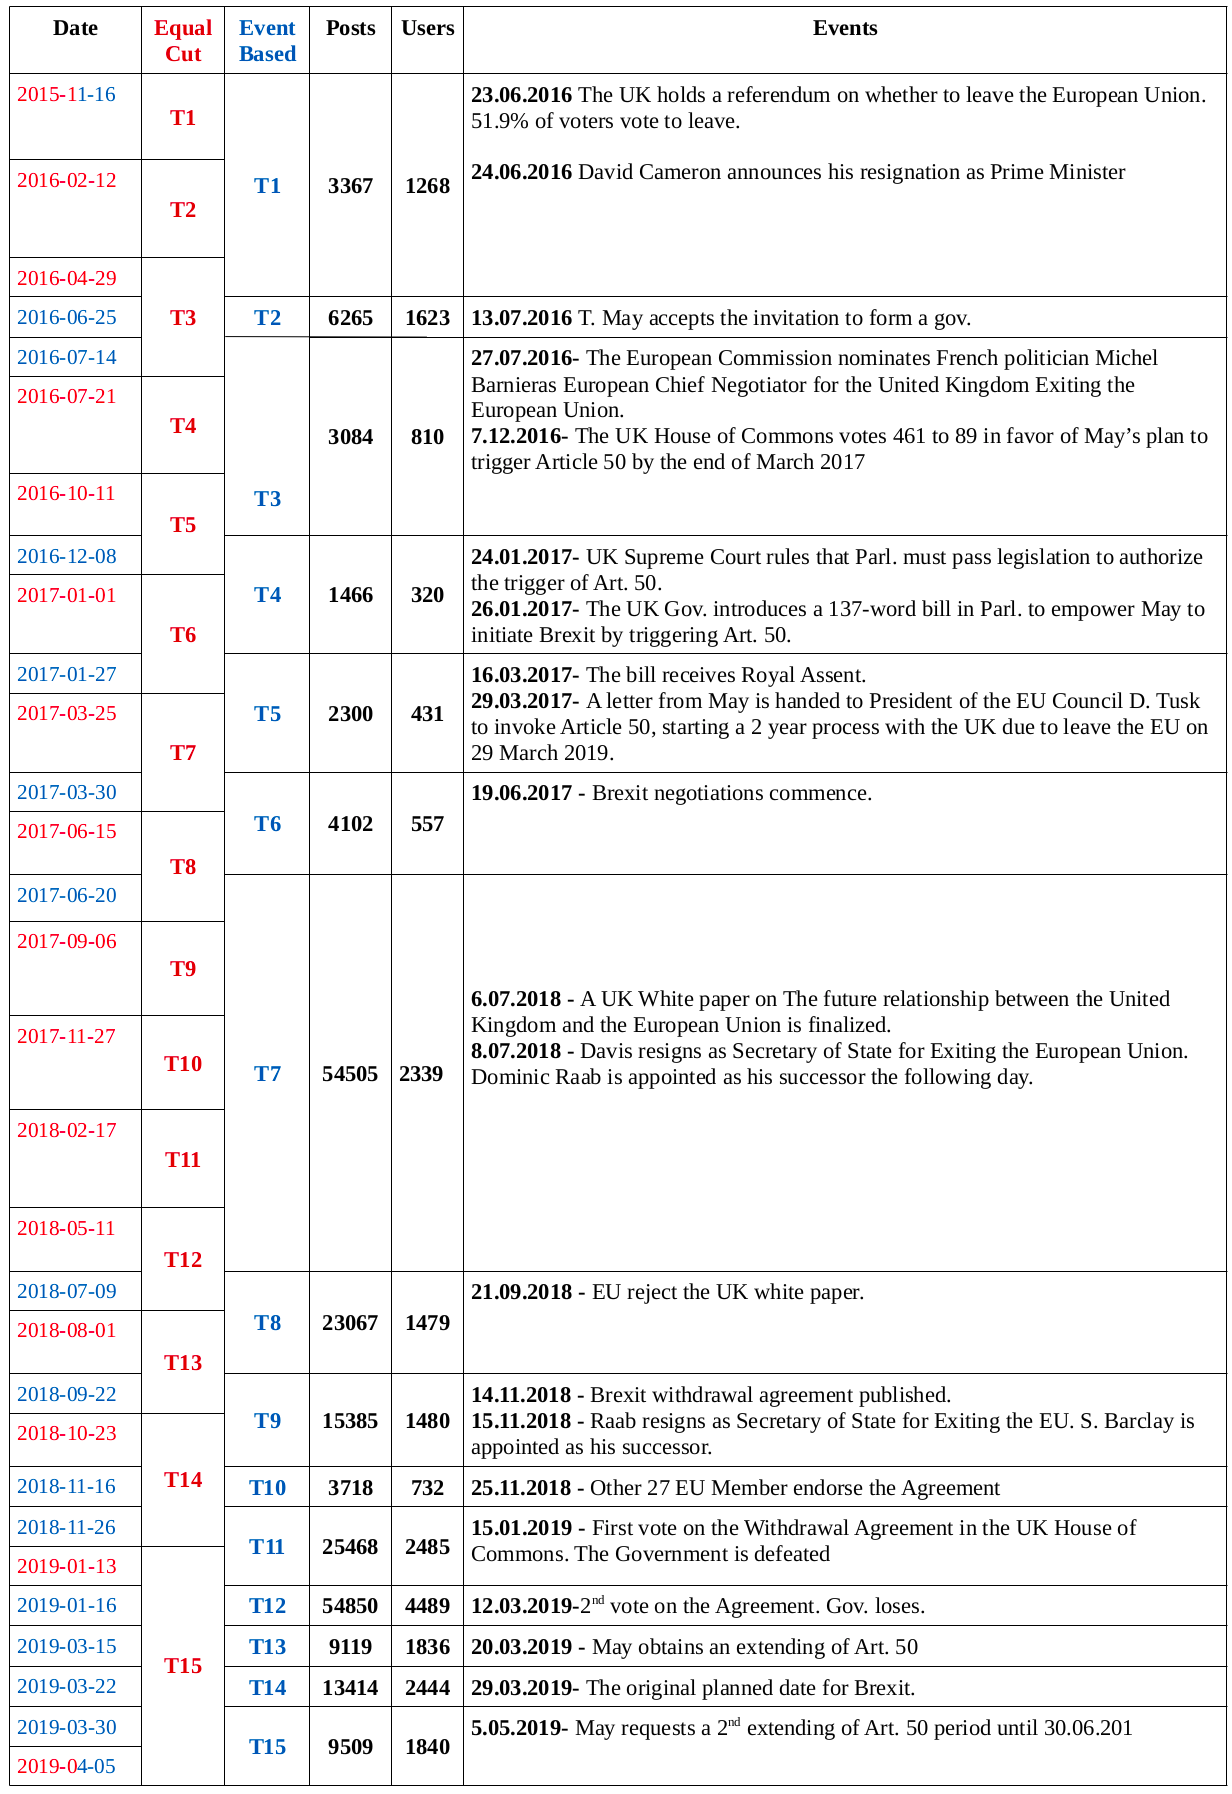
\includegraphics[width=0.93\textwidth]{per}

	\begin{tabular}{clrrp{\mywidth}}
		\toprule
		\textbf{Int.} & \multicolumn{1}{c}{\textbf{Start date}} & \multicolumn{1}{c}{\textbf{Posts}} & \multicolumn{1}{c}{\textbf{Users}} & \multicolumn{1}{c}{\textbf{Important events in the Brexit chronology}} \\ \midrule
		T1 & 2015-11-16 & 3367 & 1268 & \makecell[t{p{\mywidth}}]{
			\textbf{23 June 2016}\\
			The UK holds a referendum on whether to leave the European Union (EU). 51.9\% of voters vote to leave.\\
			\textbf{24 June 2016}\\
			David Cameron announces his resignation as Prime Minister.} \\ 
			
		T2 & 2016-06-25 & 6265 & 1623 & \makecell[t{p{\mywidth}}]{
			\textbf{13 July 2016}\\
			Theresa May accepts the Queen's invitation to form a government} \\
			
		T3 & 2016-07-14 & 3084 & 810 & \makecell[t{p{\mywidth}}]{
			\textbf{27 July 2016}\\
			The European Commission nominates French politician Michel Barnier as European Chief Negotiator for the United Kingdom Exiting the European Union.\\
			\textbf{7 December 2016}\\
			The UK House of Commons votes 461 to 89 in favour of May’s plan to trigger Article 50 by the end of March 2017} \\

		T4 & 2016-12-08 & 1466 & 320 & \makecell[t{p{\mywidth}}]{
			\textbf{24 January 2017}\\
			UK Supreme Court rules that Parl. must pass legislation to authorize the trigger of Art. 50.\\
			\textbf{26 January 2017}\\
			The UK Gov. introduces a 137-word bill in Parl. to empower May to initiate Brexit by triggering Art 50.} \\

		T5 & 2017-01-27 & 2300 & 431 & \makecell[t{p{\mywidth}}]{
			\textbf{16 March 2017}
			The bill receives Royal Assent.\\
			\textbf{29 March 2017}\\
			A letter from May is handed to President of the European Council Donald Tusk to invoke Article 50, starting a two year process with the UK due to leave the EU on 29 March 2019.} \\

		T6 & 2017-03-30 & 4102 & 557 & \makecell[t{p{\mywidth}}]{
			\textbf{19 June 2017}
			Brexit negotiations commence.} \\

		T7 & 2017-06-20 & 54505 & 2339 & \makecell[t{p{\mywidth}}]{
			\textbf{6 July 2018}\\
			A UK White paper on The future relationship between the United Kingdom and the European Union is finalized.\\
			\textbf{8 July 2018}\\
			Davis resigns as Secretary of State for Exiting the EU. Dominic Raab is appointed as his successor the following day.} \\

		T8 & 2018-07-09 & 23067 & 1479 & \makecell[t{p{\mywidth}}]{
			\textbf{21 September 2018}
			EU rejects the UK white paper.} \\

		T9 & 2018-09-22 & 15385 & 1480 & \makecell[t{p{\mywidth}}]{
			\textbf{14 November 2018}
			Brexit withdrawal agreement published.\\
			\textbf{15 November 2018}\\
			Raab resigns as Secretary of State for Exiting the EU. Stephen Barclay is appointed as his successor the following day.} \\

		T10 & 2018-11-16 & 3718 & 732 & \makecell[t{p{\mywidth}}]{
			\textbf{25 November 2018}\\
			Other 27 EU Member States endorse the Withdrawal Agreement.} \\

		T11 & 2018-11-26 & 25468 & 2485 & \makecell[t{p{\mywidth}}]{
			\textbf{15 January 2019}\\
			First meaningful vote held on the Withdrawal Agreement in the UK House of Commons. The UK Gov. is defeated by 432 votes to 202} \\

		T12 & 2019-01-16 & 54850 & 4489 & \makecell[t{p{\mywidth}}]{
			\textbf{12 March 2019}\\
			Second meaningful vote on the Withdrawal Agreement with the UK Government defeated again by 391 votes to 242.\\
			\textbf{14 March 2019}\\
			UK Gov. motion passes 412 to 202 to extend the Article 50 period.} \\

		T13 & 2019-03-15 & 9119 & 1836 & \makecell[t{p{\mywidth}}]{
			\textbf{20 March 2019}\\
			May requests the EU extend the Article 50 period until 30 June 2019.\\
			\textbf{21 March 2019}\\
			The European Council offers to extend the Article 50 period until 22 May 2019 if the Withdrawal Agreement is passed by 29 March 2019 but, if it does not, then the UK has until 12 April 2019 to indicate a way forward. The extension is formally agreed the following day.} \\
	
		T14 & 2019-03-22 & 13414 & 2444 & \makecell[t{p{\mywidth}}]{
			\textbf{29 March 2019}\\
			The original end of the Article 50 period and the original planned date for Brexit. Third vote on the Withdrawal Agreement after being separated from the Political Declaration. UK Government defeated again by 344 votes to 286.} \\
	
		T15 & 2019-03-30 & 9509 & 1840 & \makecell[t{p{\mywidth}}]{
			\textbf{5 April 2019}\\
			May requests for a second time that the EU extend the Article 50 period until 30 June 2019.} \\

		& 2019-04-05 &  &  & \textit{--dataset end--} \\ \bottomrule
	\end{tabular}

\end{table}